\documentclass{standalone}

\usepackage{tikz}
\usepackage{ctex}

\begin{document}
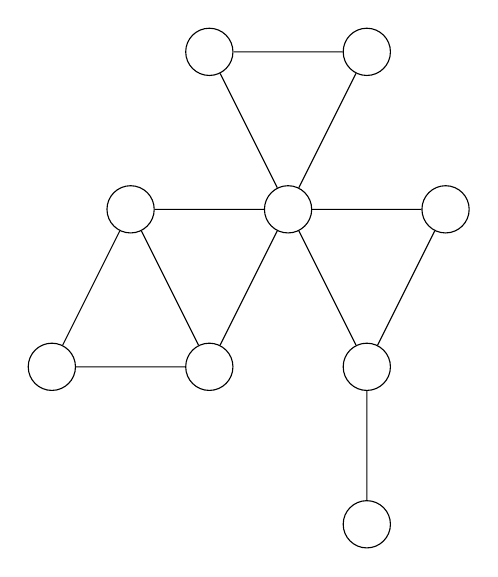
\begin{tikzpicture}[x=20mm,y=20mm]

\begin{scope}[every node/.style={draw,minimum size=6mm},circle]
    \node (A) at (-0.5,1){};
    \node (B) at (0.5,1) {};
    \node (C) at (0,0) {};
    \node (D) at (-1,0) {};
    \node (E) at (-0.5,-1) {};
    \node (F) at (-1.5,-1) {};
    \node (G) at (1,0) {};
    \node (H) at (0.5,-1) {};
    \node (I) at (0.5,-2) {};
\end{scope}

\draw
 (A) -- (B) -- (C) -- (A)
 (C) -- (D)
 (C) -- (E)
 (D) -- (E) -- (F) -- (D)
 (C) -- (G) -- (H) -- (C)
 (H) -- (I);

\end{tikzpicture}
\end{document}
